\section{Experiments}\label{sec:exp}
\subsection{Implementation Details.}
\paragraph{Training Setup.}
We use Qwen2.5-VL-3B-Instruct~\citep{bai2025qwen2} as the MLLM backbone for \method{} and all ablation variants. Following GUI-Actor~\citep{wu2025gui}, we retain the next-token prediction loss for \method{}'s grounding format. \method{}-3B is trained on 8 NVIDIA A100-80G GPUs with a global batch size of 64 and a learning rate of $5\times 10^{-6}$. We set $\alpha=0.8$ for the adaptive deviation control in Gaussian labeling. For visual-sink query token selection, we use the top-1 token under the global uniform criterion in \cref{eq:find_sink}. The patch grid resolution is $28\times 28$ in Qwen2.5-VL base model. \method{}-3B is trained for one epoch with all parameters unfrozen, without extra modules or a warm-up stage.
\begin{table*}[!t]
    \centering
    \setlength{\tabcolsep}{0.5pt}
    \caption{Performance comparison of different models across various task categories based on Text, Icon, and Average scores on {\bf ScreenSpot-Pro}. ``-'' indicates unreported results in original papers. Methods with $^*$ are Qwen2.5-VL-based. {\faSearchPlus} denotes two-step inference with zoom-in.}
    % \vspace{-1em}
    \scriptsize
    \resizebox{\textwidth}{!}{%
    % \begin{tabular}{@{} c l
    %     c c p{0.4em}
    %     c c p{0.4em}
    %     c c p{0.4em}
    %     c c p{0.4em}
    %     c c p{0.4em}
    %     c c p{0.4em}
    %     c c c @{}}
    \begin{tabular}{c l
        c c p{0.4em}
        c c p{0.4em}
        c c p{0.4em}
        c c p{0.4em}
        c c p{0.4em}
        c c p{0.4em}
        c c c}
    \toprule
    & \multirow{2}{*}{\textbf{Model}} 
    & \multicolumn{2}{c}{\textbf{CAD}} 
    & \multicolumn{1}{c}{}
    & \multicolumn{2}{c}{\textbf{Dev}} 
    & \multicolumn{1}{c}{}
    & \multicolumn{2}{c}{\textbf{Creative}} 
    & \multicolumn{1}{c}{}
    & \multicolumn{2}{c}{\textbf{Scientific}} 
    & \multicolumn{1}{c}{}
    & \multicolumn{2}{c}{\textbf{Office}} 
    & \multicolumn{1}{c}{}
    & \multicolumn{2}{c}{\textbf{OS}} 
    & \multicolumn{1}{c}{}
    & \multicolumn{3}{c}{\textbf{Average}} \\
    \cmidrule(lr){3-4}\cmidrule(lr){6-7}\cmidrule(lr){9-10}\cmidrule(lr){12-13}\cmidrule(lr){15-16}\cmidrule(lr){18-19}\cmidrule(lr){21-23}
    & & Text & Icon
    &
    & Text & Icon
    &
    & Text & Icon
    &
    & Text & Icon
    &
    & Text & Icon
    &
    & Text & Icon
    &
    & Text & Icon & \textbf{Avg.} \\
    \midrule
    \multirow{5}{*}{\rotatebox{90}{\bf General}}
    & Claude Computer~\citep{hu2024dawnguiagentpreliminary} & 14.5 & 3.7
    &
    & 22.0 & 3.9
    &
    & 25.9 & 3.4
    &
    & 33.9 & 15.8
    &
    & 30.1 & 16.3
    &
    & 11.0 & 4.5
    &
    & 23.4 & 7.1 & 17.1 \\
    & Qwen2.5-VL-3B~\citep{bai2025qwen2} & 9.1 & 7.3
    &
    & 22.1 & 1.4
    &
    & 26.8 & 2.1
    &
    & 38.2 & 7.3
    &
    & 33.9 & 15.1
    &
    & 10.3 & 1.1
    &
    & 23.6 & 3.8 &  16.1 \\
    & Qwen2.5-VL-7B~\citep{bai2025qwen2} & 16.8 & 1.6
    &
    & 46.8 & 4.1
    &
    & 35.9 & 7.7
    &
    & 49.3 & 7.3
    &
    & 52.5 & 20.8
    &
    & 37.4 & 6.7
    &
    & 38.9 & 7.1 &  26.8 \\
    & Qwen3-VL-8B~\citep{bai2025qwen3} & 56.9 & 10.9
    &
    & 75.3 & 22.8
    &
    & \underline{68.2} & 16.1
    &
    & \underline{78.5} & 32.7
    &
    & \underline{80.8} & 39.6
    &
    & \underline{71.0} & 20.2
    &
    & \bf71.1 & 22.8 &  52.7 \\
    & Qwen3-VL-30B-A3B~\citep{bai2025qwen3} & 51.8 & 15.6
    &
    & \underline{76.0} & 24.8
    &
    & \bf69.2 & 20.3
    &
    & 76.4 & 27.3
    &
    & \underline{80.8} & 37.7
    &
    & \bf75.7 & 38.2
    &
    & \underline{70.6} & 26.3 &  \underline{53.7} \\
    \midrule
    \multirow{9}{*}{\rotatebox{90}{\bf SFT}}
    & OS-Atlas-7B~\citep{wu2024atlas} & 12.2 & 4.7
    &
    & 33.1 & 1.4
    &
    & 28.8 & 2.8
    &
    & 37.5 & 7.3
    &
    & 33.9 & 5.7
    &
    & 27.1 & 4.5
    &
    & 28.1 & 4.0 &  18.9 \\
    & UGround-V1-7B~\citep{gou2024navigating} & 15.8 & 1.2
    &
    & 51.9 & 2.8
    &
    & 47.5 & 9.7
    &
    & 57.6 & 14.5
    &
    & 60.5 & 13.2
    &
    & 38.3 & 7.9
    &
    & 45.2 & 8.1 &  31.1 \\
    & UI-TARS-72B~\citep{qin2025ui} & 18.8 & 12.5
    &
    & 62.9 & 17.2
    &
    & 57.1 & 15.4
    &
    & 64.6 & 20.9
    &
    & 63.3 & 26.4
    &
    & 42.1 & 15.7
    &
    & 50.9 & 17.6 & 38.1 \\
    & \textsc{Jedi}-3B$^*$~\citep{xie2025scaling} & 27.4 & 9.4
    &
    & 61.0 & 13.8
    &
    & 53.5 & 8.4
    &
    & 54.2 & 18.2
    &
    & 64.4 & 32.1
    &
    & 38.3 & 9.0
    &
    & 49.8 & 13.7 &  36.1 \\
    & \textsc{Jedi}-7B$^*$~\citep{xie2025scaling} & 38.0 & 14.1
    &
    & 42.9 & 11.0
    &
    & 50.0 & 11.9
    &
    & 72.9 & 25.5
    &
    & 75.1 & 47.2
    &
    & 33.6 & 16.9
    &
    & 52.6 & 18.2 &  39.5 \\
    & GUI-Actor-3B$^*$~\citep{wu2025gui} & - & -
    &
    & - & -
    &
    & - & -
    &
    & - & -
    &
    & - & -
    &
    & - & -
    &
    & - & - &  42.2 \\
    & GUI-Actor-3B$^*$ + Verifier & - & -
    &
    & - & -
    &
    & - & -
    &
    & - & -
    &
    & - & -
    &
    & - & -
    &
    & - & - & 45.9 \\
    & GUI-Actor-7B$^*$~\citep{wu2025gui} & - & -
    &
    & - & -
    &
    & - & -
    &
    & - & -
    &
    & - & -
    &
    & - & -
    &
    & - & - &  44.6 \\
    & GUI-Actor-7B$^*$ + Verifier & - & -
    &
    & - & -
    &
    & - & -
    &
    & - & -
    &
    & - & -
    &
    & - & -
    &
    & - & - &  47.7 \\
    \midrule
    \multirow{11}{*}{\rotatebox{90}{\bf RL}}
    & GUI-G$^2$-3B$^*$~\citep{tang2025gui} & 20.3 & 9.4
    &
    & 42.2 & 2.1
    &
    & 43.4 & 2.8
    &
    & 43.8 & 10.0
    &
    & 46.3 & 15.1
    &
    & 29.0 & 4.5
    &
    & 37.6 & 6.0 &  25.5 \\
    & UI-R1-E-3B$^*$~\citep{lu2025ui} & 37.1 & 12.5
    &
    & 46.1 & 6.9
    &
    & 41.9 & 4.2
    &
    & 56.9 & 21.8
    &
    & 65.0 & 26.4
    &
    & 32.7 & 10.1
    &
    & - & - &  33.5 \\
    & InfiGUI-R1-3B$^*$~\citep{liu2025infiguig1advancingguigrounding} & 33.0 & 14.1
    &
    & 51.3 & 12.4
    &
    & 44.9 & 7.0
    &
    & 58.3 & 20.0
    &
    & 65.5 & 28.3
    &
    & 43.9 & 12.4
    &
    & 49.1 & 14.1 & 35.7 \\
    & SE-GUI-3B$^*$~\citep{yuan2025enhancing} & 38.1 & 12.5
    &
    & 55.8 & 7.6
    &
    & 47.0 & 4.9
    &
    & 61.8 & 16.4
    &
    & 59.9 & 24.5
    &
    & 40.2 & 12.4
    &
    & 50.4 & 11.8 & 35.9 \\
    & GUI-G1-3B$^*$~\citep{zhou2025gui} & 39.6 & 9.4
    &
    & 50.7 & 10.3
    &
    & 36.6 & 11.9
    &
    & 61.8 & 30.0
    &
    & 67.2 & 32.1
    &
    & 23.5 & 10.6
    &
    & 49.5 & 16.8 & 37.1 \\
    & InfiGUI-G1-3B$^*$~\citep{liu2025infigui} & 50.8 & 25.0
    &
    & 64.9 & 20.0
    &
    & 51.5 & 16.8
    &
    & 68.8 & 32.7
    &
    & 70.6 & 32.1
    &
    & 49.5 & 15.7
    &
    & - & - &  45.2 \\
    & UI-TARS-1.5-7B~\citep{qin2025ui}$^*$ & - & -
    &
    & - & -
    &
    & - & -
    &
    & - & -
    &
    & - & -
    &
    & - & -
    &
    & - & - &  49.6 \\
    & GroundNext-3B (RL)$^*$~\citep{feizi2025grounding} & 55.3&  32.8& &  65.6&  36.6&&   50.0&  24.5& &  66.0&  37.3 & & 74.6 & 50.9 & & 45.8 & 29.2& &  59.9&  33.6&  49.8\\
    & GTA1-7B$^*$~\citep{yang2025gta1} & \bf 66.9 & 20.7
    &
    & 62.6 & 18.2
    &
    & 53.3 & 17.2
    &
    & 76.4 & 31.8
    &
    & \bf82.5 & 50.9
    &
    & 48.6 & 25.9
    &
    & 65.5 & 25.2 & 50.1 \\
    &InfiGUI-G1-7B$^*$~\citep{liu2025infigui}&57.4& 23.4&& 74.7& 24.1&& 64.6& 15.4 &&\bf80.6& 31.8&& 75.7& 39.6 &&57.0& 29.2&& 68.4 &25.2&  51.9\\
    &GroundNext-7B (RL)$^*$~\citep{liu2025infigui}&  50.2 & 34.3& &  73.4&  40.0& &  59.6&  23.8& &  70.1 & 42.7& &  74.6 & 54.7 & & 53.3 & 30.3 & & 60.5&  33.6&  52.9\\
    \midrule
    % \multirow{4}{*}{\rotatebox{90}{\bf OURS}}
    & \textbf{\method{}-3B-lite}$^*$ & 44.7 & 21.9
    &
    & 68.2 & 28.3
    &
    & 59.6 & 21.7
    &
    & 69.4 & 37.3
    &
    & 70.6 & 49.1
    &
    & 65.4 &  31.5
    &
    & 62.0 & 30.0 & 49.8 \\
    & \textbf{\method{}-3B-lite}$^*$+ \faSearchPlus & 54.3&  26.6& & \bf 77.9 & 37.2& &  67.2&  \underline{31.5}& &  76.4 & 39.1& &  \underline{80.8}&  \underline{64.2} & & 61.7 & 32.6& &  69.5 & 36.8 &  \underline{57.0}\\
    & \textbf{\method{}-3B}$^*$ & 50.3 & \underline{34.4}
    &
    & 68.8 & \underline{46.9}
    &
    & 52.0 & 30.1
    &
    & 75.0 & \underline{43.6}
    &
    & 74.0 & 50.9
    &
    & 56.1 & \underline{39.3}
    &
    & 62.1 & \underline{40.2} &  \bf53.8 \\
    & \textbf{\method{}-3B}$^*$+ \faSearchPlus & \underline{58.4} & \bf45.3
    &
    & 73.4 & \bf48.3
    &
    & 63.6 & \bf41.3
    &
    & 77.8 & \bf47.3
    &
    & \bf82.5 & \bf66.0
    &
    & 67.3 & \bf49.4
    &
    & 70.0 & \bf47.9 &  \bf61.5 \\
    \bottomrule
    \end{tabular}
    }
    \label{tab:screenspot_pro}
\end{table*}

\paragraph{Training Data and Inference Setup.}
To examine the scalability of \method{} with increased training data, we train two model variants: \method{}-3B-lite is trained on the full training sets of GUIAct~\citep{chen2024guicourse}, AndroidControl~\citep{li2024effects}, and Wave-UI~\citep{waveui}, together with 60k randomly sampled samples from UGround~\citep{gou2024navigating} and 60k from the GTA1's training set~\citep{yang2025gta1guitesttimescaling}, resulting in 259k instructions and approximately 85k images in total. \method{}-3B is then further trained with an additional 250k instructions (509k in total) from GroundCUA~\citep{feizi2025grounding} to better scale to desktop scenarios. For the 45k ablation training set for ablations in \cref{sec:ablation}, we use the first 10k samples from GUIAct, AndroidControl, and Wave-UI, together with the first 15k samples from UGround. For the two-step inference in \cref{sec:zoom}, we set the crop size to $616$ pixels and use a $2\times$ zoom-in ratio in the second pass. Additional implementation details of \method{} and baselines are provided in \cref{app:anchor,app:baseline}.

\paragraph{Benchmarks and Metrics.}
We evaluate \method{} on five GUI grounding benchmarks covering a wide range of grounding scenarios: ScreenSpot-Pro~\citep{li2025screenspot}, OSWorld-G~\citep{xie2505scaling} and UI-Vision~\citep{nayak2025ui} (in-domain) for the desktop scenario, ScreenSpot-v2~\citep{wu2024atlas} and MMBench-GUI-L2~\citep{wang2025mmbench} for general evaluations across mobile, desktop, and web domains. 
For grounding accuracy, we follow the standard center-point metric~\citep{lin2024showui}: a prediction is considered correct if the click point falls within the ground-truth bounding box.
% \paragraph{Baselines.}Three categories of methods are compared: 
% (1) General MLLMs including
% GPT-4o~\citep{openai2024gpt4o}, 
% Gemini-2.5-Pro~\citep{comanici2025gemini}, 
% Claude Computer~\citep{hu2024dawnguiagentpreliminary},
% Operator~\citep{cua2025},
% Qwen2.5-VL~\citep{bai2025qwen2}; (2) GUI-specific supervised fine-tuned model: 
% OS-Atlas~\citep{wu2024atlas}, 
% UGround~\citep{gou2024navigating}, 
% UI-TARS~\citep{qin2025ui}, 
% JEDI~\citep{xie2025scaling} and 
% GUI-Actor~\citep{wu2025gui}
% ; (3) GUI-specific Reinforcement fine-tuned model: 
% UI-R1~\citep{lu2025ui},  
% InfiGUI-R1~\citep{liu2025infiguig1advancingguigrounding}, 
% GUI-G1~\citep{zhou2025gui}, 
% SE-GUI~\citep{yuan2025enhancing}, 
% GUI-G$^2$~\citep{tang2025gui}.
% \paragraph{Baselines.}Three categories of methods are compared: 
% (1) General MLLMs including
% Gemini-2.5-Pro~\citep{comanici2025gemini}, 
% Claude Computer~\citep{hu2024dawnguiagentpreliminary},
% Operator~\citep{cua2025},
% Qwen2.5-VL~\citep{bai2025qwen2}  and Qwen3-VL~\citep{bai2025qwen3}; (2) GUI-specific supervised fine-tuned models: 
% OS-Atlas~\citep{wu2024atlas}, 
% UGround~\citep{gou2024navigating}, 
% UI-TARS~\citep{qin2025ui}, 
% JEDI~\citep{xie2025scaling}, 
% GUI-Actor~\citep{wu2025gui} and GroundNext (SFT)~\citep{feizi2025grounding}; (3) GUI-specific Reinforcement fine-tuned models: 
% UI-R1~\citep{lu2025ui},  
% InfiGUI-R1~\citep{liu2025infiguig1advancingguigrounding}, 
% GUI-G1~\citep{zhou2025gui}, 
% SE-GUI~\citep{yuan2025enhancing}, 
% GUI-G$^2$~\citep{tang2025gui}, GTA1~\citep{yang2025gta1}, InfiGUI-G1~\citep{liu2025infigui} and GroundNext (RL)~\citep{feizi2025grounding}.

\paragraph{Baselines.}Three categories of methods are compared: 
(1) General MLLMs; (2) GUI-specific supervised fine-tuned models; (3) GUI-specific Reinforcement fine-tuned models. For our variants, \method{}-3B-lite is trained on the subset of GUI-Actor~\citep{wu2025gui}'s training data, while \method{}-3B additionally incorporates the 250k subset of GroundNext~\citep{feizi2025grounding}'s training data (710k). UI-Vision results are in-domain for both \method{}-3B and GroundNext.
\begin{table*}[!t]
    \centering
    \footnotesize
    \caption{Performance comparison on \textbf{ScreenSpot-v2}. ``-'' indicates unreported results in original papers. Methods with $^*$ are Qwen2.5-VL-based.}
    \resizebox{\linewidth}{!}{
        \begin{tabular}{clccccccc}
    \toprule
    & \multirow{3}{*}{\textbf{Model}} 
      & \multicolumn{2}{c}{\textbf{Mobile}}
      & \multicolumn{2}{c}{\textbf{Desktop}}
      & \multicolumn{2}{c}{\textbf{Web}}
      & \multirow{2.5}{*}{\textbf{Avg.}} \\
    \cmidrule(lr){3-4}\cmidrule(lr){5-6}\cmidrule(lr){7-8}
    & & Text & Icon & Text & Icon & Text & Icon &  \\
    \midrule
    \multirow{6}{*}{\rotatebox{90}{\bf General}}
    & Operator~\citep{cua2025}  & 47.3 & 41.5 & 90.2 & 80.3 & 92.8 & 84.3 & 70.5\\
    & GPT-4o~\citep{openai2024gpt4o} + OmniParser-v2~\citep{yu2025omniparserv2structuredpointsofthoughtunified} & 95.5 & 74.6 & 92.3 & 60.9 & 88.0 & 59.6 & 80.7 \\
    & Qwen2.5-VL-3B~\citep{bai2025qwen2} & 93.4 & 73.5 & 88.1 & 58.6 & 88.0 & 71.4 & 80.9 \\
    & Qwen2.5-VL-7B~\citep{bai2025qwen2} &97.6 & 87.2 & 90.2 & 74.2 & 93.2 & 81.3 & 88.8   \\
    &Qwen3-VL-8B~\citep{bai2025qwen3} &\bf 99.7 &87.7 &94.8 &83.6& \underline{95.3}& 85.7& \underline{92.1}\\
    &Qwen3-VL-30B-A3B~\citep{bai2025qwen3}& 99.0& 87.7& 95.4& 82.9& \underline{95.3} &83.7 &91.7\\
    \midrule
    \multirow{7}{*}{\rotatebox{90}{\bf SFT}}
    & OS-Atlas-7B~\citep{wu2024atlas} & 95.2 & 75.8 & 90.7 & 63.6 & 90.6 & 77.3 & 84.1\\
    & UGround-V1-7B~\citep{gou2024navigating} & 95.0 & 83.3 & 95.0 & 77.8 & 92.1 & 77.2 & 87.6 \\
    & UI-TARS-7B~\citep{qin2025ui} & 96.9 & \underline{89.1} & 95.4 & 85.0 & 93.6 & 85.2 & 91.6\\
    & \textsc{Jedi}-3B$^*$~\citep{xie2025scaling}  & 96.6 & 81.5 & \bf96.9 & 78.6 & 88.5 & 83.7 & 88.6\\
    & \textsc{Jedi}-7B$^*$~\citep{xie2025scaling} & \bf96.9 & 87.2 & 95.9 & 87.9 & 94.4 & 84.2 & 91.7 \\
    & GUI-Actor-3B~\citep{wu2025gui}& 97.6& 83.4& \bf96.9& 83.6& 94.0& 85.7& 91.0 \\
    &GUI-Actor-3B + Verifier& 98.3 & 85.3&\bf96.9 & 87.9 & 95.3 & \bf86.7 & \bf92.4\\
    \midrule
    \multirow{7}{*}{\rotatebox{90}{\bf RL}}
    & GUI-G$^2$-3B$^*$~\citep{tang2025gui} &96.5 &82.5&95.4&75.0&88.4&72.4&86.3\\
    &InfiGUI-R1-3B$^*$~\citep{liu2025infiguig1advancingguigrounding} &97.1 &81.2 &94.3& 77.1& 91.7& 77.6 &87.5\\
    &GroundNext-3B (RL)$^*$~\citep{feizi2025grounding} &94.8& \bf96.4 &93.9 &87.1 &90.6 &79.3& 88.5\\
    & UI-R1-E-3B$^*$~\citep{lu2025ui}  &98.2 &83.9& 93.2 &83.7& 94.8 &75.0 &89.5\\
    & UI-TARS-1.5-7B$^*$~\citep{qin2025ui} &95.9 &84.8 &94.9& 80.7& 90.6& \underline{86.2}& 89.7\\
    &GroundNext-7B (RL)$^*$~\citep{feizi2025grounding}& 96.6 &88.2& 95.4 &87.9& 94.9& 75.9 &90.4\\
    &InfiGUI-G1-3B$^*$~\citep{liu2025infigui} & 99.3 &88.2 &94.8& 82.9 &94.9& 80.3& 91.1\\ 
    \midrule
    & \textbf{\method{}-3B-lite}$^*$ &99.2&85.9&\underline{96.1}&\underline{88.9}&\bf96.1&80.2&91.5\\
    & \textbf{\method{}-3B}$^*$ &\underline{99.6}&84.8&95.6&\bf91.3&94.3&84.8&\underline{92.1}\\
    \bottomrule
    \end{tabular}}
    \label{tab:screenspot_v2}
\end{table*}
\subsection{Main Results: Grounding Performance}
We compare \method{} with state-of-the-art methods on ScreenSpot-Pro (\cref{tab:screenspot_pro}), ScreenSpot-v2 (\cref{tab:screenspot_v2}), UI-Vision and MMBench-GUI-L2 (\cref{tab:ui_mm}), and OSWorld-G (\cref{tab:osworld_g}).

\textbf{Desktop scenario.}
\method{} achieves strong performance on challenging high-resolution desktop benchmarks. On ScreenSpot-Pro, \method{}-3B-lite reaches 49.8\% accuracy, and additional desktop-focused training with 200k GroundCUA instructions further scales \method{}-3B to 53.8\%, outperforming strong SFT and RL baselines. Moreover, our patch-level attention grounding naturally enables a two-step zoom-in inference, which substantially improves performance to 57.0\% for \method{}-3B-lite and 61.5\% for \method{}-3B, with particularly large gains on the abstract icon subset. Despite being trained with less than one-third of the GroundCUA data used by GroundNext-3B, \method{}-3B achieves comparable in-domain performance on UI-Vision, while outperforming it on the other benchmarks. On OSWorld-G,  given already a competitive base model (62.8\%), \method{}-3B is further improved to 68.1\% with zoom-in, performing competitively against the strongest large-scale baselines (GTA1-7B and Qwen3-VL-30B-A3B). These results highlight the practical advantage of directly supervising intrinsic attention for dense, high-resolution desktop interfaces.

\textbf{General grounding across domains.}
On ScreenSpot-v2, \method{}-3B outperforms same-scale and larger baselines, and remains competitive with the two-step GUI-Actor-3B with verifier, which is trained on 9.6M samples, demonstrating the data efficiency of \method{}. Notably, \method{} achieves strong icon grounding across desktop domains, indicating robust generalization beyond text-heavy cases. On MMBench-GUI-L2, \method{}-3B consistently outperforms same-scale baselines and matches many larger models.

Overall, \method{} is both effective and scalable. The intrinsic attention grounding manner provides data efficiency for better scaling and flexibility for inference-time improvements without additional training. The consistent improvement from \method{}-3B-lite to \method{}-3B with additional single-domain data further demonstrates the scalability of intrinsic attention supervision. The improvement of \method{} over GUI-Actor shows the advantage of intrinsic attention supervision without adding an extra module and training stage, with much less training effort in a natural manner. We provide additional quantitative results on ScreenSpot-v1~\citep{cheng2024seeclick} in \cref{app:extra_res}. Qualitative visualizations of attention grounding can be found in \cref{app:example}.
\begin{table*}[!t]
    \centering
    \footnotesize
    \caption{Performance comparison on \textbf{UI-Vision} and \textbf{MMBench-GUI-L2}. ``-'' indicates unreported results in original papers. Methods with $^*$ are Qwen2.5-VL-based.}
    \resizebox{\linewidth}{!}{
        \begin{tabular}{clcccc|ccc}
    \toprule
    & \multirow{2}{*}{\textbf{Model}} 
      & \multicolumn{4}{c|}{\textbf{UI-Vision}}& \multicolumn{3}{c}{\textbf{MMBench-GUI-L2}}\\
      \cmidrule(lr){3-6}\cmidrule(lr){7-9}
    & & Basic & Func. & Spatial &\bf Avg. &Basic &Advanced&\bf Avg. \\
    \midrule
    \multirow{4}{*}{\rotatebox{90}{\bf General}}
    &Qwen2.5-VL-7B$^*$~\citep{bai2025qwen2} &1.2& 0.8& 0.5& 0.9&38.0   & 29.8    & 33.9\\
    & Qwen3-VL-2B$^*$~\citep{bai2025qwen3} & 16.4 & 19.1 & 4.6  & 13.1 & 84.3  &54.9 &69.5 \\
    & Qwen3-VL-8B$^*$~\citep{bai2025qwen3} & 27.8 & 29.6 & 9.4  & 21.9 &90.2&72.7&81.4 \\
    & Qwen3-VL-30B-A3B$^*$~\citep{bai2025qwen3} & 31.2 & 31.9 & 14.6 & 25.6&91.0&76.5&83.7 \\
    \midrule
    \multirow{7}{*}{\rotatebox{90}{\bf SFT}}
    &OS-Atlas-Base-7B~\citep{wu2024atlas}    &12.2& 11.2& 3.7& 9.0  &       52.8   &   30.1 &      41.4\\
     &Aguvis-7B~\citep{xu2024aguvis} &17.8& 18.3& 5.1 &13.7&-  &   - &      45.7 \\
    &UGround-V1-7B~\citep{gou2024navigating} &15.4 &17.1 &6.3 &12.9  &               78.4  &  53.0&     65.7 \\
    & GUI-Actor-3B$^*$~\citep{wu2025gui} &-&-&-& 19.7&-&-& 69.8\\
    & GUI-Actor-7B$^*$~\citep{wu2025gui} &-&-&-&21.9 &-&-&70.9\\
    &JEDI-7B$^*$~\citep{xie2025scaling}&-&-&-&24.8 &-&-&70.4\\
    &GroundNext-3B (SFT)$^*$~\citep{feizi2025grounding}&70.9& 59.8 &45.1 &58.2 &86.5&64.5&75.5\\
    \midrule
     \multirow{8}{*}{\rotatebox{90}{\bf RL}}
    &UI-TARS-1.5-7B$^*$~\citep{qin2025ui}&- &-  &  -   &  20.8 & 78.4   & 50.4   &  64.3 \\
    &InfiGUI-G1-3B$^*$~\citep{liu2025infigui}&31.2& 28.0& 8.2& 22.0 &84.1 &  62.9  &  73.4    \\
    &InfiGUI-G1-7B$^*$~\citep{liu2025infigui}&36.2& 31.9& 11.5& 26.1& 88.3&   73.3&    80.8\\
    &GTA1-7B$^*$~\citep{yang2025gta1}&- &-  &  -   &  25.7 &-  &  -    & 79.4 \\
    &GUI-G$^2$-7B$^*$~\citep{tang2025gui} &- &-  &  -   &  25.6 &-  &  -    & 79.5 \\
    &Holo2-8B~\citep{hcompany2025holo2} & 43.6 & 43.5 & 19.7 & 35.1 & \underline{91.7}   &\underline{77.4} &   \underline{84.5}\\
    &Holo2-30B-A3B~\citep{hcompany2025holo2}& 51.0 & 50.1 & 23.2 & 40.9&\bf92.8&\bf\bf80.7 &\bf86.8 \\
    &GroundNext-3B (RL)$^*$~\citep{feizi2025grounding}&\bf72.9 &\bf63.9 &\bf50.6& \bf62.1 &87.3&67.1&77.1\\
    \midrule
    & \textbf{\method{}-3B-lite}$^*$ &39.2 & 33.9 & 10.6 & 27.9 &86.2  &66.5 & 76.3 \\
    & \textbf{\method{}-3B}$^*$ & \underline{70.8}& \underline{63.1}& \underline{46.2} & \underline{60.0}&88.3  &69.9 &  79.1  \\     
    \bottomrule
    \end{tabular}}
    \label{tab:ui_mm}
\end{table*}

\subsection{Ablations}\label{sec:ablation}
\cref{tab:ablation} shows the ablation results on ScreenSpot-v2 and ScreenSpot-Pro. All the ablation variants are trained on the 45k ablation training data with Qwen2.5-VL-3B-Instruct as the backbone. GUI-Actor (45k) is trained in two stages same as the original setting. Additional ablations trained on the 259k training set of \method{}-lite are shown in \cref{app:extra_abla}.

\paragraph{Compare Coordinate-free modeling manners.} In \cref{tab:ablation}, we include 3 different coordinate-free GUI grounding manners, one embedding-based: GUI-Actor, which relies on hidden embeddings for computing similarity with extra modules, and two attention-based: vanilla attention grounding as \cref{eq:aggre_vanilla} and simplified attention grounding as \cref{eq:aggre_final}. With the same importance on all the query tokens and attention heads, the vanilla attention grounding can converge faster than GUI-Actor on more complex visual grounding tasks in ScreenSpot-Pro. When simplifying the aggregation on query tokens, even with naive "weighting uniformly", the simplified attention grounding can have \textbf{1.50\%} and \textbf{4.24\%} improvement over GUI-Actor for ScreenSpot-v2 and ScreenSpot-Pro. These results demonstrate the effectiveness and faster convergence of attention-based visual grounding methods than embedding-based methods, and show the advantage of compressing query contexts into $\texttt{<ANCHOR>}$ token instead of manually controlling the grounding importance from each query token. 
% \input{sec/tab_ablation}

\paragraph{GUI grounding without Visual-sink Query Token $\mathcal{Q}_s$.} For attention-based GUI grounding variants, weighting the query-visual correlation of each head via the cumulative sum of all query's predictions as $\mathcal{Q}'=\mathcal{Q}$ (TAG's manner) or only the prediction from $\texttt{<ANCHOR>}$ as $\mathcal{Q}'=\{\texttt{<ANCHOR>}\}$ in \cref{eq:unified_head_score} leads to more biased attention predictions than uniform weighting, with worse ScreenSpot-v2 performance of both variants and no improvement on ScreenSpot-Pro as shown in ``Attention Head Weighting without $\mathcal{Q}_s$ in \cref{eq:unified_head_score}'' part of \cref{tab:ablation}. This bias comes from the misleading weighting from visual-unrelated tokens for the variants using all $\mathcal{Q}$ and from using the premature $\texttt{<ANCHOR>}$ token for grounding in the later variant. 

 \begin{table*}[!t]
    \centering
    \footnotesize
    \caption{Performance comparison of different models across various task categories based on Mobile, Desktop, Web and Average scores on \textbf{OSWorld-G-Refine}. Methods with $^*$ are Qwen2.5-VL-based. {\faSearchPlus} denotes two-step inference with zoom-in.}
    % \vspace{-1em}
    \resizebox{\linewidth}{!}{
    \begin{tabular}{clccccc} 
    \toprule
    & \textbf{Model} % 'Model' will now be centered
      & \makecell{\textbf{Text}\\\textbf{Matching}}    % Split into two lines
      & \makecell{\textbf{Element}\\\textbf{Recognition}} % Split into two lines
      & \makecell{\textbf{Layout}\\\textbf{Understanding}}% Split into two lines
      & \makecell{\textbf{Fine-grained}\\\textbf{Manipulation}} % Split into two lines 
      & {\textbf{Avg.}} \\
    \midrule 
    \multirow{6}{*}{\rotatebox{90}{\bf General}}
    & Operator~\citep{cua2025}  &  51.3& 42.4& 46.6& 31.5& 40.6  \\
    & Gemini-2.5-Pro~\citep{comanici2025gemini} & 59.8 &45.5& 49.0& 33.6 &45.2 \\
    & Qwen2.5-VL-3B~\citep{bai2025qwen2} &41.4 &28.8 &34.8 &13.4& 27.3\\
    & Qwen2.5-VL-7B~\citep{bai2025qwen2} & 45.6& 32.7 &41.9 &18.1 & 31.4  \\
    &Qwen3-VL-8B~\citep{bai2025qwen3} &78.2& 71.5 &72.3& 55.7&67.0\\
    &Qwen3-VL-30B-A3B~\citep{bai2025qwen3} &77.8 &\underline{75.8} &\underline{74.7}& 54.4& \bf69.3\\
    \midrule
    \multirow{7}{*}{\rotatebox{90}{\bf SFT}}
    & OS-Atlas-7B~\citep{wu2024atlas} & 44.1 &29.4& 35.2 &16.8 & 27.7 \\
    & UGround-V1-7B~\citep{gou2024navigating} & 51.3 &40.3& 43.5& 24.8 &36.4  \\
    & UI-TARS-7B~\citep{qin2025ui} & 60.2& 51.8& 54.9 &35.6 &47.5 \\
    & \textsc{Jedi}-3B$^*$~\citep{xie2025scaling} & 67.4 &53.0 &53.8 &44.3 &50.9 \\
     & \textsc{Jedi}-7B$^*$~\citep{xie2025scaling} &65.9& 55.5& 57.7 &46.9 & 54.1  \\
     & GUI-Actor-3B$^*$~\citep{wu2025gui}  &64.4&   60.6&  64.8  &33.6   &54.6	\\
     & GUI-Actor-7B$^*$~\citep{wu2025gui}  &65.9&	62.7&	66.4&	38.2	&56.6	\\
    \midrule
    \multirow{6}{*}{\rotatebox{90}{\bf RL}}
    &SE-GUI-7B$^*$~\citep{yuan2025enhancing} &-&-&-&-&33.9\\
    &InfiGUI-G1-3B$^*$~\citep{liu2025infigui}& 65.5& 53.0& 56.1& 34.2&49.6\\
    &InfiGUI-G1-7B$^*$~\citep{liu2025infigui}& \underline{72.0}& 63.6& 66.8& 46.3 &59.9\\
    &GUI-G$^2$-7B$^*$~\citep{liu2025infigui} &-&-&-&-&61.9\\
    &UI-TARS-1.5-7B$^*$~\citep{qin2025ui} & 52.6& 75.4& 72.4& \underline{66.7}& 64.2 \\
    &GTA-1-7B$^*$~\citep{yang2025gta1}& 63.2& \bf82.1 &74.2 &\bf70.5 &  67.7\\
    \midrule
    & \textbf{\method{}-3B-lite}$^*$ &64.8&65.5&68.8&36.8&58.3\\
    & \textbf{\method{}-3B-lite}$^*$+ \faSearchPlus&71.3&70.6&73.1&47.4&63.8 \\
    & \textbf{\method{}-3B}$^*$&67.4&	71.2&	72.7&	39.5&	62.8 \\
    & \textbf{\method{}-3B}$^*$+ \faSearchPlus&\bf72.4&	\underline{75.8}&	\bf78.7&	48.7&	\underline{68.1} \\
    \bottomrule
    \end{tabular}}
    % \vspace{-2em}
    \label{tab:osworld_g}
\end{table*}
\begin{table*}[!t]
    \centering
    \footnotesize
    \begin{minipage}[t]{0.56\textwidth}
        \centering
    \caption{Ablation results on ScreenSpot-v2 and ScreenSpot-Pro of coordinate-free GUI grounding methods fine-tuned with a 45k ablation dataset. Variants in \colorbox{blue!10}{blue} represent the selected settings for \method{}.}
    % \vspace{-0.5em}
    \resizebox{\linewidth}{!}{
    % \begin{tabular}{y{160}cccccc}
    \begin{tabular}{p{160pt}cccccc}
        \toprule
        \multirow{2}{*}{\textbf{Model}} & \multicolumn{3}{c@{\hspace{1em}}}{\textbf{ScreenSpot-v2}$\uparrow$} & \multicolumn{3}{c@{\hspace{1em}}}{\textbf{ScreenSpot-Pro}$\uparrow$}\\
        & Text & Icon & \textbf{Avg.}& Text & Icon & \textbf{Avg.} \\
        \midrule
        \rowcolor{gray!30} 
        \multicolumn{7}{l}{\textit{Existing Coordinate-free GUI Grounding}} \\
        GUI-Actor-3B (45k) & 96.24 & 75.99 & 87.42 & 50.67 & 12.25 & 35.99 \\
        Vanilla Attention Grounding (45k) & 95.68 & 75.45 & 86.87 & 53.02 & 12.42 & 37.51 \\
        \midrule
        \rowcolor{gray!30} 
        \multicolumn{7}{l}{\textit{Simplified Attention Grounding: GUI-AIMA-3B (45k)}} \\
        \rowcolor{gray!10}\multicolumn{7}{l}{\textit{Attention Head Weighting without $\mathcal{Q}_s$} in \cref{eq:unified_head_score}}\\
        + weighting uniformly & 97.08 & 78.34 & 88.92 & 56.50 & 13.91 & 40.23 \\
        + weighting with all $\mathcal{Q}'=\mathcal{Q}$ & 96.24 & 78.34 & 88.44 & 52.61 & 13.41 & 37.63 \\
        + weighting with $\mathcal{Q}'=\{\texttt{<ANCHOR>}\}$ & 96.66 & 76.35 & 87.81 & 56.91 & 14.57 & 40.73 \\
        \rowcolor{gray!10}\multicolumn{7}{l}{\textit{Attention Head Weighting with }$\mathcal{Q}'=\mathcal{Q}_s$\textit{ in} \cref{eq:unified_head_score}}\\
        + layer-wise $\operatorname{top-1} \mathcal{Q}_s^l$ & 96.52 & \textbf{81.23} & \textbf{89.86} & 57.32 & \underline{15.73} & 41.43 \\
        + layer-wise $\operatorname{top-3} \mathcal{Q}_s^l$ & 96.66 & 79.06 & 88.99 & 57.83 & \underline{15.07} & 41.49 \\
        \rowcolor{blue!10}
        + global $\operatorname{top-1} \mathcal{Q}_s$ & \textbf{97.49} & 78.88 & 89.39 & \underline{59.26} & 14.40 & \underline{42.13} \\
        + global $\operatorname{top-3} \mathcal{Q}_s$ & 95.82 & 70.94 & 84.98 & 57.01 & 14.40 & 40.73 \\
        \rowcolor{blue!10}
        ~~~~ + weighted patch-wise labeling & \underline{97.21} & \underline{79.60} & \underline{89.54} & \textbf{61.00} & 14.90 & \textbf{43.39} \\
        \bottomrule
      \end{tabular}}
    % \vspace{-2em}
    \label{tab:ablation}
\end{minipage}
    \hfill
    \begin{minipage}[t]{0.4\textwidth}
    \captionsetup{type=figure}
    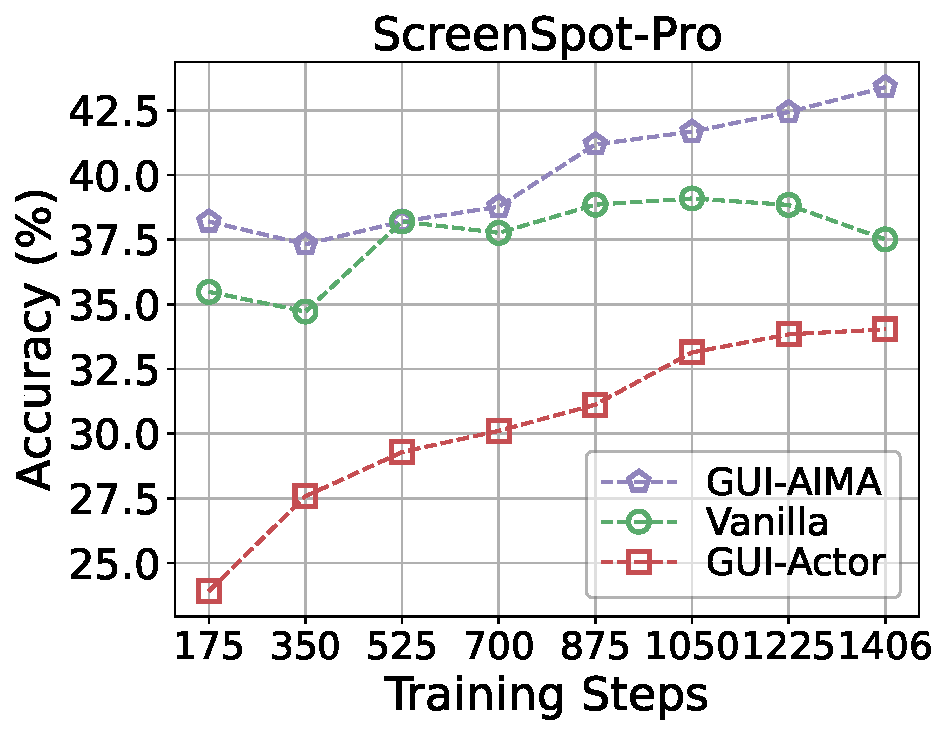
\includegraphics[width=\linewidth]{fig/convergence_ablation.pdf}
    \vspace{-2em}
    \caption{Model convergence of the 45k ablation dataset on ScreenSpot-Pro benchmark. %of \method{}, GUI-Actor and vanilla attention grounding.
    }
    \label{fig:Convergence}
    \end{minipage}
\end{table*}
\begin{table*}[!t]
    \centering
    \footnotesize
    \begin{minipage}[t]{0.56\textwidth}
        \centering
    \caption{Analysis experiment results on ScreenSpot-pro. \textbf{Relax@k} measures how many previously incorrect offset predictions are recovered when the ground-truth bounding box is expanded by k visual patches along each dimension. \textbf{Corrected} refers to the number of offset predictions corrected by the second step, while \textbf{Lost} refers to the number of predictions that degrade after the second step.}
    % \vspace{-0.5em}
    \resizebox{\linewidth}{!}{
    % \begin{tabular}{y{160}cccccc}
    \begin{tabular}{lcccc|cc|c}
        \toprule
        Model& Relax@1 & Relax@3 & Relax@5 & \textbf{Total} & \textbf{Corrected} & \textbf{Lost}&\textbf{Improved} \\
        \midrule
        \rowcolor{gray!30}
        \multicolumn{8}{l}{\textit{1-step}} \\
        Origin 1-step & 158 & 92 & 56 & 306 & - & - &-\\
        \midrule
        \rowcolor{gray!30}
        \multicolumn{8}{l}{\textit{2-step}} \\
        Crop-only & 123 & 83 & 43 & 249 & 156 & 107 &49\\
        Crop + 1.5$\times$Zoom-in & 47 & 74 & 38 & 159 & 208 & 48 & 160\\
        Crop + 2$\times$Zoom-in& 39 & 63 & 45 & 147 & 215&33& \bf 182  \\
        Crop + 3$\times$Zoom-in& 39 & 69 & 44 & 152 &219 & 42&177 \\
        Crop + 4$\times$Zoom-in& 31 & 72 & 38 & 141 &224 & 48&176\\
        \bottomrule
      \end{tabular}}
    % \vspace{-2.5em}
    \label{tab:analysis_zoom}
\end{minipage}
    \hfill
    \begin{minipage}[t]{0.4\textwidth}
    \captionsetup{type=figure}
    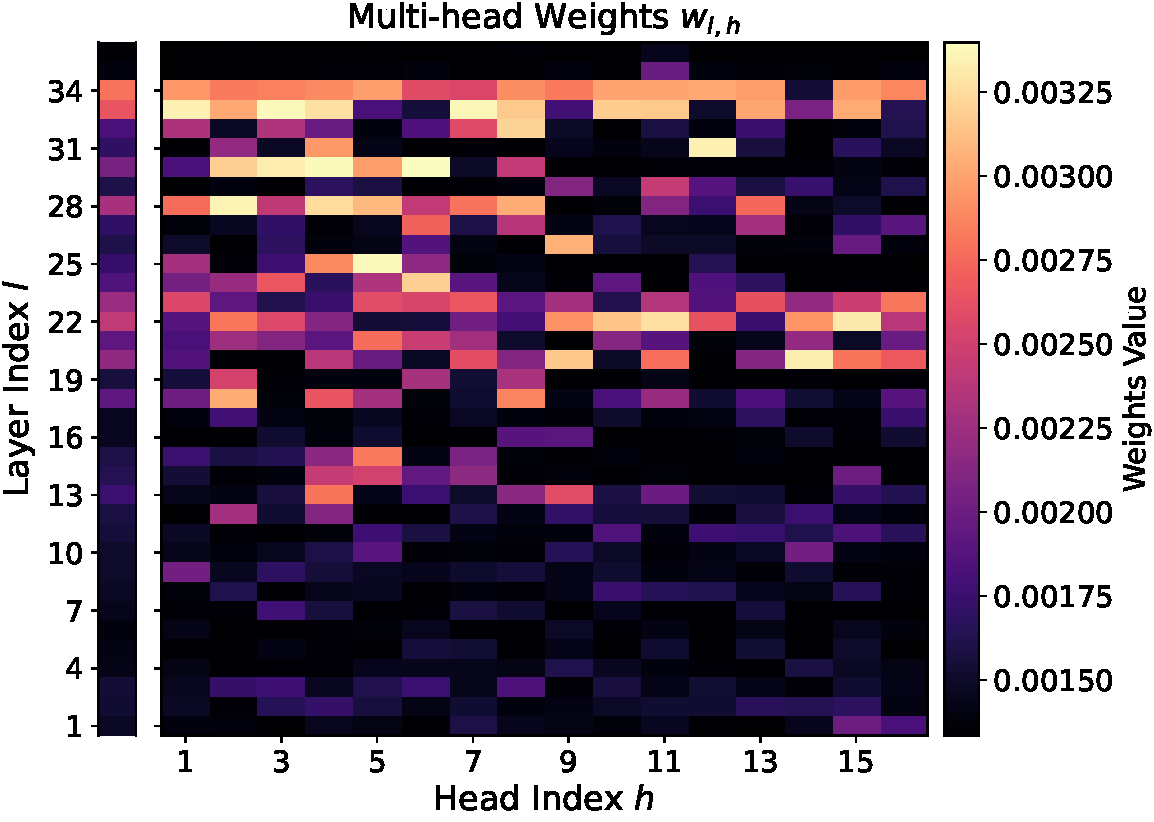
\includegraphics[width=0.9\linewidth]{fig/ALL_mean_headweights.pdf}
    \vspace{-1em}
    \caption{Visualization of multi-head weights $w_{l,h}$ averaged over the ScreenSpot-Pro, ScreenSpot-v2 and OS-World-G. \textbf{Left:} layer-wise mean, i.e., for layer $l$: $\frac{1}{H}\sum_{h=1}^{H}w_{l,h}$. \textbf{Right:} per-layer, per-head weights $w_{l,h}$.
    }
    \label{fig:contribution_head}
    \end{minipage}
\end{table*}
\paragraph{The effect of Visual-sink Query Token $\mathcal{Q}_s$.} For ablation of using $\mathcal{Q}_s$ for $w_{l,h}$, we vary the $\operatorname{K}$ value between 1 and 3 in the $\operatorname{topK}$ selection of $\mathcal{Q}_s$ tokens and explore whether differing $\mathcal{Q}_s^l$ for each MLLM's layer, i.e., $\mathcal{Q}_s^l\coloneqq \operatorname*{arg\,topK}_{q_i\in\mathcal{Q}}(c_{q_i}^{\,l})$, or using the same $\mathcal{Q}_s$ for all layers as in \cref{eq:find_sink}. In \cref{tab:ablation}, we can observe that the layer-wise manner performs slightly better on the icon-based tasks, but uniformly-selected same $\mathcal{Q}_s$ for all layers leads to more balanced results on both text and icon sets. Among both manners, $\operatorname{top-1}$ selection remains the overall best performance. These ablations verify the ``global $\operatorname{top-1} \mathcal{Q}_s$'' setting of \method{}, with \textbf{1.90\%} improvement over ``weighting uniformly'' on ScreenSpot-Pro.

\paragraph{Patch-wise labeling considering overlapping and distance.} Here, we also justify the overlapping- and distance-aware~\citep{tang2025gui} patch-wise labeling for fine-tuning \method{} in \cref{eq:labeling}. Based on ``global $\operatorname{top-1} \mathcal{Q}_s$'', down-weighting partial positive and distanced image patches instead of labeling all patches equally leads to \textbf{1.26\%} further enhancement on ScreenSpot-Pro.

\paragraph{Training efficiency.} In \cref{fig:Convergence}, we show the convergence tendency of three methods: \method{}, vanilla attention grounding and GUI-Actor (with extra warm-up stage already) initialized from Qwen-2.5-VL-3B. \method{} converges fastest and achieves the best final results, with steady improvements. Vanilla attention grounding fluctuates as supervision on all tokens from the pretrained vocabulary impairs the general capacity. And GUI-Actor needs a longer training period to customize its extra modules for GUI grounding. 
\subsection{Analysis of Two-step Inference with Zoom-in}\label{sec:zoomin_analysis}
In \cref{tab:analysis_zoom}, we present the analysis results of the two-step inference with zoom-in introduced in \cref{sec:zoom}. The analysis focuses on incorrect offset predictions, where the predicted center points fall outside the ground-truth bounding box by a small degree. \cref{tab:analysis_zoom} reports the statistics of offset errors for one-step and two-step inference with different offset distances, and the number of {Corrected} predictions as well as the {Lost} originally-correct predictions after applying the second crop-and-zoom-in step. 
We observe that performing inference on the focused region determined by the first-step prediction already corrects more than a 18.6\% samples (57) with ``Crop-only'' operation, arising from fewer irrelevant patches showing as distracting noise for our patch-wise grounding. And after cropping, zooming in by a factor from 1.5× to 4× significantly reduces offset errors, especially those with slight deviation (Relax@1). It also helps resolving large-offset errors, achieving up to 31\% (29 fixed) and 32\% (18 fixed) error reduction for Relax@3 and Relax@5, respectively. From the analysis results, we find that the performance of two-step inference is not very sensitive to the zoom-in factor, while a 2-time zoom-in provides the best performance.
\subsection{Attention Head Contribution in GUI Grounding}
In \cref{fig:contribution_head}, we visualize the head weights $w_{l,h}$ used during inference of \method{}. Overall, higher weights concentrate in mid-to-late layers (e.g., 22, 28, 33, 34), indicating that deep layers' representations contribute more to grounding. Mid layers contain highly dominant heads (e.g., head 25-5), whereas late layers (e.g., layer 34) tend to exhibit a broader set of moderately high-weight heads.

To quantify the effect of head selection, we perform inference-time head pruning based on $w_{l,h}$. Preserving only the top 30\% heads produces nearly unchanged accuracy (91.0\% on ScreenSpot-v2 and 53.5\% on ScreenSpot-Pro). In contrast, preserving only the bottom 30\% heads causes a substantial drop (76.6\% on ScreenSpot-v2 and 38.1\% on ScreenSpot-Pro). These results confirm that $w_{l,h}$ serves as an effective indicator of grounding-relevant attention heads. 